\pdfoutput=1

\documentclass{l4proj}
\usepackage{listings}
\usepackage{textcomp}
\usepackage{xcolor}
\usepackage{url}
\usepackage{stackengine}
\usepackage [english]{babel}
\usepackage [autostyle, english = american]{csquotes}
\usepackage{courier}
\MakeOuterQuote{"}


\begin{document}


%Set the Font/Coloring for the GPC language,
%Use the C++ default with added seq and par keywords
\makeatletter
\lstdefinestyle{myGPC} {language=C++,
                basicstyle=%
                \ttfamily
                \lst@ifdisplaystyle\scriptsize\fi,
                keywordstyle=\color{blue}\ttfamily,
                stringstyle=\color{red}\ttfamily,
                commentstyle=\color{gray}\ttfamily,
                morecomment=[l][\color{magenta}]{\#},
                directivestyle={\color{green}},
                identifierstyle=\color{purple},
                numbers=left,
                showstringspaces=false,
                morekeywords={seq, par, begin}
}
\makeatother



\makeatletter
\lstdefinestyle{myGPIR} {language=Lisp,
                basicstyle=%
                \ttfamily
                \lst@ifdisplaystyle\scriptsize\fi,
                keywordstyle=\color{blue}\ttfamily,
                commentstyle=\color{gray}\ttfamily,
                morecomment=[l][\color{magenta}]{\#},
                identifierstyle=\color{purple},
                numbers=left,
                showstringspaces=false,
                morekeywords={seq, par, begin},
                deletekeywords={write, read}
}
\makeatother


\makeatletter
\lstdefinestyle{myHaskell} {language=Haskell,
                basicstyle=%
                \ttfamily
                \lst@ifdisplaystyle\scriptsize\fi,
                keywordstyle=\color{blue}\ttfamily,
                stringstyle=\color{red}\ttfamily,
                commentstyle=\color{gray}\ttfamily,
                morecomment=[l][\color{magenta}]{\#}
                directivestyle={\color{green}}
                identifierstyle=\color{purple},
                numbers=left,
                morekeywords={seq}
}
\makeatother


\makeatletter
\lstdefinestyle{myJava} {language=Java,
                basicstyle=%
                \ttfamily
                \lst@ifdisplaystyle\scriptsize\fi,
                keywordstyle=\color{blue}\ttfamily,
                stringstyle=\color{red}\ttfamily,
                commentstyle=\color{gray}\ttfamily,
                morecomment=[l][\color{magenta}]{\#}
                directivestyle={\color{green}}
                identifierstyle=\color{purple},
                numbers=left,
                morekeywords={seq}
}
\makeatother


\newcommand\YAMLcolonstyle{\color{red}\mdseries}
\newcommand\YAMLkeystyle{\color{black}\bfseries}
\newcommand\YAMLvaluestyle{\color{blue}\mdseries}

\makeatletter

% here is a macro expanding to the name of the language
% (handy if you decide to change it further down the road)
\newcommand\language@yaml{yaml}

\expandafter\expandafter\expandafter\lstdefinelanguage
\expandafter{\language@yaml}
{
  keywords={true,false,null,y,n},
  keywordstyle=\color{darkgray}\bfseries,
                basicstyle=%
                \ttfamily
                \lst@ifdisplaystyle\scriptsize\fi,
  sensitive=false,
  comment=[l]{\#},
  morecomment=[s]{/*}{*/},
  commentstyle=\color{purple}\ttfamily,
  stringstyle=\YAMLvaluestyle\ttfamily,
  moredelim=[l][\color{orange}]{\&},
  moredelim=[l][\color{magenta}]{*},
  moredelim=**[il][\YAMLcolonstyle{:}\YAMLvaluestyle]{:},   % switch to value style at :
  morestring=[b]',
  morestring=[b]",
  literate =    {---}{{\ProcessThreeDashes}}3
                {>}{{\textcolor{red}\textgreater}}1     
                {|}{{\textcolor{red}\textbar}}1 
                {\ -\ }{{\mdseries\ -\ }}3,
}


\title{Design and Compilation of a C-like front-end language for GPRM}
\author{Ross Meikleham}
\date{March 2015}
\maketitle


\educationalconsent

\tableofcontents

% --- Main Content ---
%\pagenumbering{arabic}
\setlength{\parindent}{0pt}

\chapter{Introduction}

\pagenumbering{arabic}
\section{GPRM}

\subsection{What is the GPRM}

The Glasgow Parallel Reduction Machine is a virtual machine framework for multi-core programming using a task-based approach. It allows the programmer to structure their programs as a separation of task-code (written as C++ classes) and communication code. 

Communication code is currently written in a language called GPIR (Glasgow Parallel Intermediate Representation). 
GPIR code controls how tasks communicate with one another and whether groups
of tasks can be evaluated sequentially or in parallel.  GPIR code is compiled down further to GPRM byte-code which is evaluated by the GPRM virtual machine.

The GPRM uses task nodes which consists of a task kernel and a task manager.

Task code is represented as a task kernel. A task kernel is a self contained unit, typically represented as a C++ class.
To create a task kernel, the C++ class needs to be in the \textit{GPRM::Kernel} name-space.

Communication code is represented as a task manager. A task manager "co-ordinates" communication between one or more task kernels, and
is represented as a function which can be called from a C++ program.\cite{GPRM}


When building, the GPRM packages the Task Kernels with 
GPRM generic code into a library. During this process the compiler analyses all classes and methods in the
Task Kernels and maps them to numeric constants. This process allows GPIR code to call Task Kernels.
GPIR code is also compiled down to GPRM byte-code packaged into the library. A serial C++ program when compiled is then linked to
this library and a call to the GPRM's "run" method executes the GPRM byte-code. 

\newpage

\begin{figure}[ht]
\pdfimageresolution=110
\begin{center}
\includegraphics{graphs/gprm.png}
\caption{A simple overview of the GPRM framework}
\end{center}
\end{figure}

\subsection{The GPIR language}

The GPIR language is a purely functional S-expression based language that is evaluated in parallel by default 
with optional sequential evaluation semantics.

Tasks in GPIR are post-fixed with a thread number to indicate to the GPRM runtime which thread
the task should run on. For example a simple GPIR program which adds numbers in parallel:

\begin{lstlisting}[style=myGPIR]
(begin
    +[0] (+[0] '3 '2) (+[1] '4 '10)
)
\end{lstlisting}

The two nested additions are performed in parallel, with the first being mapped onto thread 0,
and the second being mapped onto thread 1. When they've both been evaluated, then the outer addition
will add the results on thread 0.

\subsubsection{Quoting}

Like in Scheme and Lisp, quoting an expression defers the evaluation of it. 
This is useful for performing sequential evaluation.

\begin{lstlisting}[style=myGPIR]
(seq 
    '(obj.m1[0] '1)
    '(obj.m2[0] '2)
)
\end{lstlisting}

Due to the parallel evaluation of GPIR, if the expressions in the seq block weren't quoted then
they would get evaluated in parallel instead of being deferred to be evaluated by the seq function.

Also literal values don't need to be evaluated, they should be deferred and passed to tasks which is
the reason the numbers are quoted in these examples.

\subsubsection{Registers}

The GPRM has registers which can be written to or read from.

\begin{lstlisting}[style=myGPIR]
(seq
    '(reg.write[0] '1 obj.m1[0])
    '(obj.m2[0] (reg.read[0] '1))
)
\end{lstlisting}

This program writes the result of the \texttt{obj.m1} call to register 1,
then reads the result from register 1 and passed it into the \texttt{obj.m2} call.

The GPIR language has other keywords and features but these are the ones that are important for
understanding the examples and design choices made for this project.

\section{Project Aims}

The GPIR language isn't really suitable for programming in. For one it requires the programmer to manually
manage which thread each task is allocated to. The language is also inconsistent with the C++ language used for 
the other parts of the framework (Calling code and Class Kernels). A language closer to C/C++ is more
consistent with the entire framework.

The aim of this project is to design a C-like language which can be evaluated in parallel by default, and build
a compiler for it. The compiler should be able to compile this new language down to GPIR code. The new language will
be called " Glasgow Parallel C" or "GPC" for short.

The language should be easy to pick up and write programs in for anyone familiar with the C/C++ languages.
To achieve this the language should be as close to C/C++ as possible. 

The language should also abstract away the details of allocating tasks to threads, this job
should be part of the compiler.


\section{Current C/C++ Parallel Programming Models}

By researching available C/C++ parallel programming frameworks/language extensions 
we can determine possible features and design choices that may suitable for the GPC language.

\subsection{Cilk Plus}

Cilk Plus is a general purpose programming language based on Cilk++\cite{cilk++}. It extends the C++ language with features such as
parallel for loops and spawning functions in parallel using a "fork-join" model to achieve task-parallelism.

One of the main principles of the Cilk language is that abstraction is important and that the programmer should use provided constructs to expose 
the parallelism in their application. This allows the programmer to be free to focus on what the code is allowed to execute in parallel and not worry about the underlying details of manually managing threads. The run-time should then have the responsibility of scheduling the threads and dividing work between
processors.\cite{cilkfaq}. 

Cilk Plus introduces 3 new keywords on top of the C++ language\cite{cilk}: 
\begin{itemize}
    \item \textit{cilk\_for} - Parallelizing for loops, uses the exact same syntax as the standard C++ for-loop
                             with some restrictions.
    \item \textit{cilk\_spawn} - Indicate that a given function can run in parallel with the remainder
                              of the calling function. 
    \item \textit{cilk\_sync} - Wait for all spawned calls to finish.
\end{itemize}

Cilk Plus applications have "serial semantics"\cite{cilk}, this means that the results of an application run
in parallel with Cilk Plus would be exactly the same if it were run
serially (\textit{cilk\_spawn} becoming a function call, removing \textit{cilk\_sync} statements, 
and replacing \textit{cilk\_for} with ordinary for loops).

Cilk Plus makes use of pragmas to indicate to the compiler that a for loop contains data parallelism.\cite{cilkfaq}

Cilk Plus also introduces a new operator \textbf{[:]} to select array sections\cite{cilkarray}. This operator
allows for "high level" operations to be performed on arrays, and can help the compiler vectorize parts of code.

The Cilk Plus runtime makes use of "task stealing" for dynamic load balancing\cite{cilkfaq}. This 
means that if one thread is idle the scheduler can reassign work assigned to be completed by a busier thread. 
The outcome of this is that the programmer doesn't have to worry about the specifics of which threads
to map tasks to, and it can be left to the runtime itself.



\section{Open MP}

OpenMP (Open Multi-Processing) is a language extension available for C, C++ and Fortran which allows for shared memory multi-processing. 
This is achieved by the use of compiler directives (more specifically in C/C++ this is done through the preprocessor using pragmas). 
This allows a compiler which doesn't implement OpenMP extensions to still compile C/C++ code
and run it in a linear fashion, and serial code can be made parallel purely through the use of preprocessor
directives without modification to the actual source code.  

\subsection{Intel TBB}

Intell TBB (Intell Thread Building Blocks) is a portable C++ template library for task parallelism.
It contains a range of concurrent algorithms, containers, and it's own task scheduler to achieve this\cite{tbb}.

Operations are treated as tasks, and the task scheduler has the job of dynamically allocating these tasks 
to individual cores which abstracts the specific details of allocating threads from the Programmer. Like CilkPlus,
Intell TBB's task scheduler also implements task stealing for dynamic load balancing\cite{tbbschedule}.

Intell TBB relies on generic programming which allows for writing parallel algorithms based on 
requirements on types. Parallel code can be written once and can work with lots of different
types without having to rewrite the algorithm for each type \cite{tbbbenefits}.

\section{Wool}
Wool\cite{wool} is a library which is inspired by Cilk that supports task parallel programming by introducing three forms of synchronization. (Create, Exit, and Join). It relies on tasks having low overheads. The 




The goal is to create a C-like language which then compiles down to GPIR code.
The language should be as C-like as possible ideally we would like it to be as much
of a complete subset of C++ as possible, as the reset of the framework (Task Kernels and calling code)
are written in C++ and is more consistent with how the entire framework works.

C++ is a statically typed, imperative language which is sequentially evaluated by default.
GPIR is a dynamically typed functional language which is evaluated in parallel by default.
Both of these are pretty much complete opposite so the language design has to be one of that
is like C++ and can be mapped onto GPIR without too much trouble.

Design decisions:

    Parallel Evaluation:
        GPIR is parallel evaluated by default, with a "seq" function which
        evaluates the given arguments in parallel. Making GPC abide by equivalent rules of parallel
        evaluation by default with optional sequential makes the most sense, and gives the
        power to do stuff. 

    Purely Functional:
        
        To allow for mapping tasks to different cores efficiently
        at compile time, the execution path must be able
        to be known at compile time. 
        
        For example given a tree-like
        recursion, 
        
        Single variable assignment
        and not allowing return values from kernel functions
        to be used in condition statements allow for this.

        To achieve this results from kernel functions are implicitly
        "tainted" as a kernel type.

        For example:
            int x = kernelObj.m1();
        has a return type of int.
        But the compiler implicitly casts this to a 
        kernel int.

        Kernel types can be passed to kernel methods, and even
        mixed with non kernel types when passed as arguments to
        kernel methods. For example:

        int y = 5;
        seq {
            int x = kernelObj.m1();
            kernelObj.m2(x + y);
        }

        would be allowed, but the following:

        int y = kernelObj.m1();



Language Features:

    This section explains the features of the language with respect to the design decisions above.

    Syntax:
        The syntax aims to be as close to C/C++ as possible. Statements must end with a semicolon. 
        All variables must be statically typed. Blocks are surrounded in braces. Case is dependent.

    New Operators:
        Two new operators not currently present in C++ "seq" and "par" are introduced. 
        These are placed before a block
        of statements to determine whether each individual statement within the block are
        to be evaluated in sequential or parallel. By default a block of statements are evaluated
        in parallel, but the par keyword makes it more explicit especially if there's lots of nested
        seq/par blocks.

    Types:
        C++ types such as string, char, bool, int, and double are included.
        Pointers, and multi-level pointer types are included.
        However pointers are restricted in that you cannot take
        an address of any variable, adding and subtracting integers
        from pointers is allowed. Usually pointers are passed into
        the GPRM from the C++ caller to represent an Array.
        
    Operations:
        Most basic binary arithmetic operations are included i.e. 
        (+, -, *, /, \%, ==, !=, &&, ||, <<, >>, &, |, ^) and
        unary operations :
        (-, ~, !) 
        are included. 

        (+=, ++, --, -=) are not included, due to the single assignment rule.
        Although an exception is made for the "afterthought" of the for loop construct, in which
        the integer loop variable can be incremented with += or decremented by -=.

    Functions:
        Exactly the same as C/C++ 


    Single assignment:
       Variables in GPC can only be assigned once per scope.

       for example the following wouldn't be allowed
           int i = 0;
           int i = i + 1;

       but the following would be:
           int i = 0;
           {
               int i = i;
           }

    For-Loops:
       For loops have the same syntax as C/C++ for loops with some restrictions.
       Essentially these are unrolled at compile-time and every iteration is evaluated in parallel.
       
       Essentialy the syntax is for(int var = n; [Boolean expression]; var += n or var -= n) 

\chapter{Implementation}


\section{Implementation Language Choice}

The compiler is implemented in the Haskell programming language.

During complication the need to traverse trees usually occurs quite
often. Functional languages like Haskell are suited to this task 
due to features such as pattern matching and tail-end recursive optimization 
which make traversing trees efficient and simple to implement.

The Glasgow Haskell Compiler is available for most platforms, most importantly for Windows, OSX and Linux 
on x86 architectures. This allows the compiler to be portable across these platforms provided the libraries 
used to build the compiler are portable.

Haskell has support for algebraic data types, these makes ASTs(Abstract Syntax Trees)
simpler to implement. For example the AST for a very simple expression
can be represented as follows:

\begin{lstlisting}[style=myHaskell]

    data Expression =
          Add Expression Expression
        | Negate Expression 
        | Const Integer

\end{lstlisting}

The equivalent in an Imperative/OOP language (in this case Java)
would be the following:

\begin{lstlisting}[style=myJava]

abstract Class Expression {}

class Add extends Expression {
    public Expression left;
    public Expression right;
    public Add(Expression l, Expression r) {
        left = l;
        right = r;    
    } 
}

class Negate extends Expression {
    public Expression expr;
    public Negate(Expression e) {
        expr = e;    
    }
} 

class Const extends Expression {
    public int value;
    public Const(int v) {
        value = v;
    }
}       

\end{lstlisting}

The Haskell version is much clearer on the structure of the tree, and takes much
less code to implement. 

It is also to easily extend Haskell data types to include
custom annotations. For example storing the source code position for parts of expressions 
which is useful for reporting errors to the user.

Due to the pure function nature of Haskell, parts of compilation can easily be performed in parallel.
For example during type checking each GPC function can be type checked in parallel and this can even be subdivided 
further into blocks within functions. For this project speed of compilation is not a major concern, but in the future if compilation ever
needs to be faster then this option is always available.

Haskell also has powerful libraries for parsing source code such as Parsec which is a parser combinator
library. Parsec allows combinator parsers to be written in the Haskell language itself avoiding the complexity
of integration of different tools and languages\cite{parsec}. 

\section{Tools and Testing}


\subsection{Cabal}

Cabal (Common Architecture for Building Applications and Libraries) is a system for building and
packaging Haskell libraries and programs\cite{cabal}. This system can manage the
project library dependencies, and automatically download and install missing dependencies.
It can also build and install the compiler on the system, and run unit tests.

\subsection{Testing}

For Unit testing the HUnit\cite{hunit} library will be used, this can be integrated
with Cabal to easily run all the required unit tests.

One form of testing used for this project is testing each individual component
(e.g. The Parser or the Type Checker). Each component in the compiler can easily
be uncoupled from one another due to the linear nature of compilation.

Another form of testing is writing GPC source files which should compile, and
GPC files which should fail compilation at a certain stage. The compiler
is then invoked during testing on all of these files to check whether
all the source files which should compile do in fact compile with no errors,
and all the source files which should raise an error do not compile.

An upside to this method is that testing this way is flexible in that
tests aren't coupled with the implementation internals of the compiler.
The only way that these test would need to be changed was if the design
of the language itself would need to be changed.

A downside to this method is that without manually checking the errors raised
by the tests that should fail; the source may generate an error which is unrelated
to the error that is being tested. This is why some testing of each internal
component is done alongside this method.

\subsection{Code Coverage}

The Haskell HPC\cite{hpc} (Haskell Program Coverage) library allows for recording
code coverage over different modules during testing. This can be integrated with
cabal unit testing to automatically generate these results. The usefulness of this
allows for checking which sections of code still need to be tested and assists
in writing further unit tests.


\section{Compiler Structure}
Compilation is split up into multiple stages or "passes",
it is possible to compile in one pass but separating each 
specific section of compilation allows modularity and decoupling.

\begin{figure}[!htb]
\begin{center}
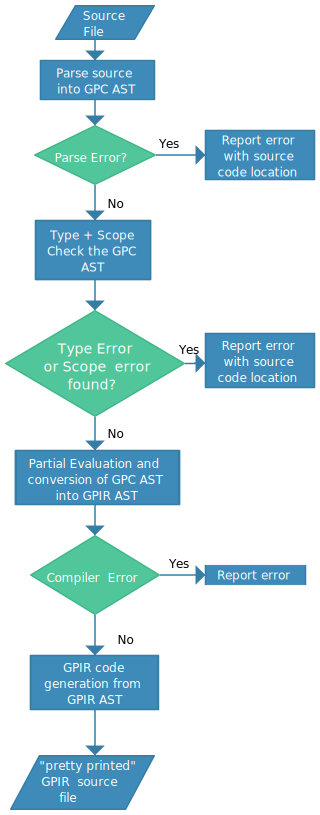
\includegraphics[scale=0.55]{graphs/Dissertation.pdf}
\caption{Flowchart illustrating the stages of the GPC compiler.}
\end{center}
\end{figure}

    
\section{Parser/Lexer}
The Parsec library combines Parsing and Lexing into one stage.

Given the GPC source file the intention is to parse the file into an AST
to hopefully eventually be transformed into GPIR source code. It's
also useful to store the original source position to provide error information 
during a further compilation stage, to achieve this the source position
info is read from Parsec into an Annotated AST as the tree is being built up.

Parsec does most of the work during this stage, including
providing error messages for "expected" values to be found in source
positions and source position information. Most of the work implementing
this stage is building the parser combinator functions and composing
them together to be able to build the AST.


\section{Type and Scope checking}
\label{sec:type}
During type checking the types of identifiers from the current scope being used in expressions need
to be known. Since the scope needs to be kept track of while type checking it makes reasonable
sense to check for scope errors in the same stage.

The goal of this stage is to ensure that the static typing of the source file
is enforced (e.g. attempting to assign a bool value to a variable of type int should not happen) and,
prevent "logic" errors at compile time (e.g. adding 2 bool values together). Scope checking
is also important as identifiers being used within the program need to be binded to an expression of
some sort, and the "single assignment" rule in the GPC language needs to be enforced.

There are two separate "types" of scope in a GPC program. The first is the top level scope and the
other is at function level scope. Any scope "further" down from function level scope is itself
a function level scope. During this stage the top level scope is type and scope checked.
Afterwards each individual function is type and scope checked.

For checking over top level statements the following Haskell record is used
to keep track of identifier types, objects, and functions encountered:

\begin{lstlisting}[style=myHaskell]
type VarTable = M.Map (Ident SrcPos) (Type SrcPos)
type FunTable = M.Map (Ident SrcPos) (Type SrcPos, [Type SrcPos])
type ObjectTable = M.Map (Ident SrcPos) (Objects SrcPos)

data MainBlock = MainBlock {
    _tlFuncDefs      :: FunTable, -- ^ Function Definitions
    _tlVarTypes      :: VarTable,  -- ^ Top Level Constant variable types
    _objects         :: ObjectTable  -- ^ Table of current Kernel objects declared 
} deriving (Show)
\end{lstlisting}

The type checker needs to check that the are no instances of duplicate functions or 
duplicate top level variables. Once this is done, and details of functions and top level
variables have been stored, each individual function can be type checked.

A slightly different structure is needed to type check functions.

At any point in time the type checker needs to know the following:
\begin{itemize}
    \item Variables that are currently in scope, and their types
    \item Functions that are available to call, their argument types, and return types
    \item Objects that are available to call methods on
    \item The current function the type checker is in
\end{itemize}

These values are stored using the following Haskell record: 

\begin{lstlisting}[style=myHaskell]

data CodeBlock = CodeBlock {
    _currentFun :: Ident SrcPos, -- ^ Name of Function block is in
    _funcDefs   :: FunTable, -- ^ Function names and return/argument types
    _prevVars   :: VarTable, -- ^ Identifiers visible in current scope with types
    _curVars    :: VarTable  -- ^ Identifiers declared in current scope
} deriving (Show)


\end{lstlisting}

When a function is being type checked a new CodeBlock instance is
created from a MainBlock instance as some of the top level information is needed.
The details of the function that is being entered is stored in \texttt{\_currentFun}, 
details of all available functions are stored in \texttt{\_funcDefs}, and all top
level variables are stored in \texttt{\_prevVars}. \texttt{\_curVars} is left 
as an empty map as the type checking of the function hasn't begun yet. Top level objects are also
stored in \texttt{\_curVars} as an "object" variable type.

Whenever a new scope is encountered by either calling a function, or entering a seq/par block;
a new CodeBlock structure is created using the current structure. The new \texttt{\_curVars}
is set to the empty map as no variables have been encountered yet, the \texttt{\_funcDefs}
are copied as all functions are on the top level so they don't change. The \texttt{\_currentFun}
is copied if entering a block, otherwise if entering a function the function name
and source position are copied. 

The value of the new \texttt{\_prevVars} is a little more complicated to work out.
Any key-value pairs in the current \texttt{\_curVars} are stored plus any key-value pairs in the 
current \texttt{\_prevVars} in which the key isn't present in the current 
set of \texttt{\_curVars} keys. This is because
the identifiers in \texttt{\_curVars} scope are visible over the identifiers with
the same name in \texttt{\_prevScope}. Haskell's union operation on maps
discards the key-value pairs in the second map for keys that are
present in the first map, so this is trivial to implement.

When type checking a function every statement in the function is type checked.
For every statement every expression within the statement is type checked, this is 
implemented by traversing the Statement AST and checking the scopes of identifiers as well 
as checking expected types match the actual types of each expression.

Objects which are declared are not checked to see if they actually exist. Neither
are method calls which means the argument types and return types when calling them
cannot be determined at compile time. This is due to the fact Objects are instantiated from
C++ classes. The C++ class of the object would need to be checked for 
methods available as well as argument and return types. 
This is already implemented in the GPRM, so an error will occur further down to compile "chain" or during
runtime.

If a type or scope error is encountered, an error message determining the type of error,
and the source position of the error is returned. Otherwise an empty tuple is returned.
When type and scope checking the original AST doesn't need to be modified, only verified
that it follows the type and scope rules of the language.


\section{Interpreting}
\label{sec:interp}

The goal of this stage is to run through the execution path the GPIR code
will take from the entry function, and partially evaluate the code as much
as possible while generating the GPIR AST. This stage involves
\textbf{Sparse Conditional Constant propagation} (\textbf{SCC}) like optimizations.

\textbf{SCC}\cite{sccp} is an optimization algorithm applied in compilers. It involves removing
dead code and performing \textbf{Constant Propogation} which involves replacing
identifiers which can be evaluated to constant values at compile time with
those values. As well as evaluating the results of constant expressions and
further propagating them. Usually this involves interpreting
the AST. How this stage differs from purely performing \textbf{SCC} optimizations
is that a new
AST is also being generated as expressions are being evaluated. Also branches 
are always able to be evaluated at compile time. Due to these reasons this
section of the build process is called "interpreting". However
\textbf{SCC} can only be applied to an immediate representation (in this case an AST)
which is in \textbf{Static Single Assignment form} (\textbf{SSA}). 

\textbf{SSA}\cite{sccp, brandis94} 
requires that every variable is assigned exactly once and is defined before being
used. The GPC language already enforces single assignment, and that variables are assigned
when they are defined (see section ~\ref{sub:single}). 
Scope checking in section ~\ref{sec:type} proves that all variables used in
the GPC AST passed to the interpreter have been defined. Therefore the GPC
AST given to the interpreter is already in \textbf{SSA} form.

Just before interpreting the GPC AST is transformed slightly into a similar AST
with a couple of differences. One is that annotations are not present (since source position information
is not needed anymore), and type information is stripped (since the program has been proven to 
not have any type errors), also objects in the top level scope are stripped (since scope checking
proved that all methods are called on objects that exist, and whenever a method is called, the
name of the object is part of the call).

Initially the values of all top level assignment statements need to be stored
as constants before executing, as well as the details for every function.

While interpreting a state is needed to determine actions taken
during certain sections, as well as to evaluate expressions.
The following Haskell record is used:

\begin{lstlisting}[style=myHaskell]

type ConstVarTable = M.Map Ident Literal
type FunTable = M.Map Ident ([Ident], BlockStmt)
type VarRegTable = M.Map Ident Integer

-- ^ Current State of the Block we are currently in
data CodeGen = CodeGen {
   _funTable    :: FunTable,  -- ^ Store symbol tree for functions
   _constTable  :: ConstVarTable, -- ^ Store constants in scope
   _varId       :: Integer, -- ^ Current variable id for mapping to registers
   _varRegTable :: VarRegTable, -- ^ maps variable identifier
   _threadCount :: Integer, -- ^ Current thread number to map
   _maxThreads  :: Integer,  -- ^ Maximum number of threads
   _seqBlock    :: Bool, -- ^ Whether or not current block is sequential
   _isReturning :: Bool -- ^ Whether the state of the current block is in a return
}

\end{lstlisting}


\subsection{Registers}
Values which can be fully evaluated at compile time can be substituted into the
GPIR code with their literal value when they are used.

For example:

\begin{center}{\textbf{GPC Code}}
\end{center}

\begin{lstlisting}[style=myGPC, frame=single]
seq {
    int x = 4 * 5;
    obj.m1();
    obj.m2(x + 3);
}
\end{lstlisting}

\begin{center}{\textbf{Compiled down to GPIR code}}
\end{center}

\begin{lstlisting}[style=myGPIR, frame=single]
seq (
     '(obj.m1[0]) 
     '(obj.m2[0] '23)
)
\end{lstlisting}

The value of \texttt{x} is able to be calculated to be 20, so whenever
\texttt{x} is used in the scope it can simply be replaced with the literal \texttt{20}.

However, some variables will not be able to be fully evaluated at compile time.
So results will have to be written to GPIR registers.

For example:

\begin{center}{\textbf{GPC Code}}
\end{center}
\begin{lstlisting}[style=myGPC, frame=single]
seq {
    int x = obj.m1();
    obj.m2(x);
}
\end{lstlisting}

\begin{center}{\textbf{Compiled down to GPIR Code}}
\end{center}
\begin{lstlisting}[style=myGPIR, frame=single]
seq (
     '(register.write[0] '1 'obj.m1[0]) 
     '(obj.m2[0] (register.read[0] '1))
)
\end{lstlisting}

The value of \texttt{x} can't be known at compile time so it is written into register \texttt{1},
and then read from the same register when it is needed.

During interpreting, there needs to be no conflict between registers (e.g. if a value
is stored in register 1 that will need to be used later, register 1 cannot be written to
until that value is out of scope). There's no hard limit on registers so a simple
method of just incrementing the register count every time a value needs to be stored
is implemented, although this may possibly cause a lot of unnecessary memory usage.

\texttt{\_varRegTable} is used to store the mappings of variable names to register numbers. 
Conflicts between variables with the same name in different scopes is not a problem,
as the register table in the inner block is thrown away once the scope is left.

\subsection{Sequential And Parallel Block Differences}
A sequential block translates to something different in GPIR than a parallel block.

For example, these two snippets compile to different GPIR code despite
the blocks containing the same code:

\begin{minipage}{.48\textwidth}
\center \textbf{GPC Parallel}
\begin{lstlisting}[style=myGPC, frame=single]
par {
    obj.m1();
    obj.m2();
}
\end{lstlisting}

\center \textbf{GPIR Parallel}
\begin{lstlisting}[style=myGPIR, frame=single]
(par obj.m1[0] obj.m2[1])
\end{lstlisting}
\end{minipage}
\hfill
%
%
\begin{minipage}{.48\textwidth}
\center \textbf{GPC Sequential}
\begin{lstlisting}[style=myGPC, frame=single]
seq {
    obj.m1();
    obj.m2();
}
\end{lstlisting}

\center \textbf{GPIR Sequential}
\begin{lstlisting}[style=myGPIR, frame=single]
(seq `obj.m1[0] `obj.m2[1])
\end{lstlisting}
\end{minipage}
 
Sequential statements need to be quoted, which is why the record contains
the \texttt{\_seqBlock} flag, so the interpreter can generate the correct GPIR code.

\subsection{Thread Mapping}
Each task in the GPRM must be mapped to a thread. There is a function
in the Interpreter called \texttt{getThread} which calculates what the next thread 
number should be to map the task to based on the current block state.

Currently this function uses a simple incremental scheme and rolls around
modulo style after the max number of threads have been specified. The compiler
attempts to work out the maximum number of cores on the machine if a thread
number isn't given, and uses this number to determine the max number of threads.

If a different scheme is needed the contents of the function will need to be changed,
a possible future improvement may be to pass a function to the interpreter when passing
it the AST to determine the counting scheme. This would allow for multiple different schemes
to be chosen and possibly tuned depending on the type of application.


\subsection{Branching}
When encountering an if statement the interpreter must be able to evaluate the condition and generate a
true or false value. The interpreter will only evaluate the statement within the if statement
if the condition is true. In the case of an if-else statement either the first statement will
be evaluated or the else statement depending on the value of the condition.


\subsection{Returning From Functions}
Performing a return is a bit tricky. 

Some pre-evaluation is needed  on blocks of statements when entering a 
new block. if a return statement is
in the current block of statements (not counting sub-blocks) then
any statements after that are "removed" and when a return statement
is found, it is evaluated as the return expression.
What this means is that once the return is met the interpreter
"returns" back to the code which executed the previous scope.

There are also two different scenarios when performing a return:

\begin{enumerate}
    \item \textbf{The interpreter is at the top level scope of a function}.
            Returning is simple in this case, all that is needed to be done is
            going to the previous scope.

    \item \textbf{The interpreter is nested within one or more blocks in a function}.
            Returning in this case involves going up multiple times until the interpreter
            is out of the scope of the current function.
\end{enumerate}

To deal with these situations a "boilerplate" function is used. This function
is called whenever an inner-scope needs to be interpreted. It
takes a boolean value which determines if the current block scope is at
the "top" of a function, gets the current state and then interprets the block.
Once the interpreter returns from interpreting the inner block, the "\_isReturning"
flag is checked on the returned state. If it is set, and the scope
of the current block is at the top of a function, then the "\_isReturning" flag
is then set for the current block.
 
When the "\_isReturning" flag is set for a block, the evaluator will not evaluate
any further statements in the current block. This allows for propagation of a "return"
up the block states until the current function is exited.


\subsection{Interpreting Functions}
When a function is called, each argument identifier in scope
is replaced by the the expression which was supplied to the function.
Then each statement in the function is evaluated.

\begin{lstlisting}[style=myGPC]

void fun(int a) {
    obj.m1(a);
    seq {
        int a = 10;
        obj.m3(a);
    }    
}

fun(5 * 4);

\end{lstlisting}

In this example when evaluating the functional call with the argument \texttt{(5 * 4)},
every \texttt{a} which is the same instance as the one in the function arguments
is replaced by the expression \texttt{(5 * 4)}. The nested \texttt{a} is not the same
instance and is not substituted.


\subsection{For Loop Evaluation}

For evaluating and unrolling for loops each loop statement needs to be evaluated
until the loop variable doesn't satisfy the condition. 

\begin{itemize}
\item The iterate function in Haskell can be used to infinitely apply the afterthought function
of the loop to generate loop variable values for each iteration.

\item Then values are taken from this list and are applied to the loops condition until
one fails. This creates a list of loop variables values for all iterations. 

\item This value list is then mapped to the statements in the loop body replacing any instance
of the loop variable. This unrolls the loop.

\item Then each statement is then evaluated. 
\end{itemize}


It is also possible to detect cases of infinite loops based on the loop variable, 
the conditional, and afterthought statements, before attempting to unroll the loop.

For example the following for loop will loop infinitely (ignoring overflow of integers, which is undefined in most C/C++ standards).
\begin{lstlisting}[style=myGPC]
for (int i = 0; i < -1; i++) {
    obj.m1(i);
}
\end{lstlisting}


\subsection{Partial Expression Evaluation}
\label{sub:partial}

There are two parts needed to evaluate an expression:

\begin{enumerate}
    \item \textbf{Constant Propogation}\cite{sccp} - All identifiers in the expression which have a value in the constant table are
          replaced with the respective constant value.

    \item \textbf{Constant Folding}\cite{sccp} - Attempt to evaluate as much of the expression with replaced constants as possible

\end{enumerate}

Replacement is trivial, using the constant table for the current scope the
expression AST is recursively travelled and any instances of identifiers
in the constant table are replaced.


Reduction is a bit more complex, it involves attempting to apply the binary
and unary operations to their respective expressions. Expressions can be
represented in a binary expression tree. Binary operators are contained in
the inner nodes with 2 children, unary operators contained in the inner
nodes with 1 child. Leaf nodes contain literal values and variables.

For example the expression \texttt{5 * 3 - 2 + \textasciitilde2} when read in by the
compiler is represented by the following tree:

\begin{center}
\includegraphics[scale=0.5]{graphs/impleval.pdf}
\end{center}


The tree is evaluated through
post-order traversal. Once two leaf nodes are found the binary operation in the parent node
is attempted to be applied to the two leaf nodes, or if one leaf node is found
with no other node the unary operation in the parent node is applied
to the leaf.  

In the case of a binary operation if both leaf nodes are values which
can be calculated at compile time the expression is evaluated, the two leaf nodes
are removed and the parent node is replaced with the calculated value. If one or
more leaf nodes are values which can only be known at runtime then the expression is
not evaluated and the tree doesn't change. 

In the case of a unary operation if the leaf node is a value which can be calculated
at compile time the expression is evaluated, otherwise the expression is not evaluated
and the tree doesn't change.

However this method isn't optimal when some sub-expressions cannot be
evaluated at compile time. In this case the expression can be fully evaluated
to a single value,
but depending on the expression this method can at times reduce the expression
down to an expression which can still be further reduced.
This problem and a possible solution is discussed in Chapter ~\ref{ch:future}.



\section{GPIR Code Generation}

Once the interpreter is completed it should produce the GPIR AST, 
from this AST the goal is to output GPIR source code.
Since the GPIR language is very simple this task is not too difficult.,
It involves recursively travelling the tree, ensuring lists containing task operations
are surrounded by parentheses, printing quotes when needed, etc.

For this task a "pretty printer" library is used which allows for formatting
the output much easier than manipulating strings. The generated GPIR source code
is saved into a file with the same prefix as the source but with a ".td" (Task Description)
extension.

\chapter{Conclusion}

\section{Benchmarks}

A merge sort algorithm has been implemented in GPC for 80 million integers with a cutoff value 
of 2048. The actual sorting and merging is performed by the \texttt{MergeSort} kernel class
methods \texttt{MergeSort.serial\_ms} and \texttt{MergeSort.merge\_two}. The GPC code structures
how the Kernel tasks should interact and calls them in parallel.\\ 

\lstinputlisting[style=myGPC]{code_samples/GPRM_MergeSort.gpc}

This code is compiled into GPIR code by the compiler from the command line by entering \texttt{gpcc GPRM\_MergeSort.gpc --threads=240}
where the \texttt{threads} argument is an optional to manually adjust the number of total threads that are available
to map tasks onto.

\newpage

\begin{figure}[!htb]
\pdfimageresolution=110
\includegraphics{graphs/benchmark.png}
\caption{Merge sort benchmarks for parallel frameworks \cite{GPRMBench}}
\label{fig:bench}
\end{figure}

The compiler compiles the merge sort GPC code into GPIR code identical to the GPIR code used to generate figure ~\ref{fig:bench}.
The \texttt{MergeSort} C++ Kernel class is also the same one used. From the figure it can easily be seen that the GPRM
far outperforms Cilk, TBB, and OpenMP on the XeonPhi, and OpenMp on the TILEPro64 for 240 threads in this specific example. 

Another thing to note is that the GPC code is a lot "nicer" than the code for the Cilk, TBB, and OpenMP
implementations, as it is almost completely pure C++.  It doesn't require the learning of how to use pragmas, 
or fork-join mechanisms.

\begin{figure}[!htb]
\pdfimageresolution=110
\includegraphics{graphs/mergebad.png}
\caption{Mergesort implementations in TBB, OpenMP, and CilkPlus \cite{GPRMBench}}
\label{fig:bench}
\end{figure}



\section{Summary}
The main goal of the project was to create a C-like language for the GPRM.
I believe that goal has been met as the language designed and implemented 
in this project is a purely functional parallel evaluation language which is an exact subset of C++ 
(apart from the two extra keywords). The language can be partially evaluated and compiled down to GPIR code 
which can be further compiled to be run on the GPRM. 

Methods and techniques that can be applied to interpret and partially evaluate purely
functional code have also been explored.

This project also leaves a lot of opportunities for future work. Compilers and Programming Languages in general have
multiple areas where there are constantly improvements to be made, most notably in language features and optimisations 
for code generation. A couple of possible improvements are explored in Chapter ~\ref{ch:future}.






\chapter{Future Work}

Future Features that could be added:
    yml config generation.
    These files are needed by the GPRM to determine aliases in GPIR code, libraries used,
    number of threads/nodes. There is enough information at compilation time to generate these,
    and they are currently generated manually. 

    Other C++ language features, C++11 lambdas may be useful,
    while-loops, and possibly some STL support e.g. ability to use STD vector instead of pointers.





%%%%%%%%%%%%%%%%%%%%
%   BIBLIOGRAPHY   %
%%%%%%%%%%%%%%%%%%%%

\bibliographystyle{ieeetr}
\bibliography{bib}

\end{document}
